\section{Hardware}\label{sec:optimalHardware}
As part of the requirements stated in \autoref{ssec:problemRequirements}, our vehicle should be car-like and host an on-board AV system.
When aiming for a car-like vehicle, some sort of \textit{propulsion} (and steering) is implied, and, to fulfill our requirements for the AV system, some sort of \textit{computing platform} is needed, as well as a \textit{world input}.
All three headlines are further described in this section.

\subsection{Propulsion Platform}\label{ssec:optimalHardwarePropulsion}
A candidate for a combination of chassis, wheels, propulsion, steering, and room for additional hardware, is the \textit{Traxxas TRX-4 Chassis Kit} \cite{TraxxasTRX4}.
\begin{figure}[H]
  \centering
  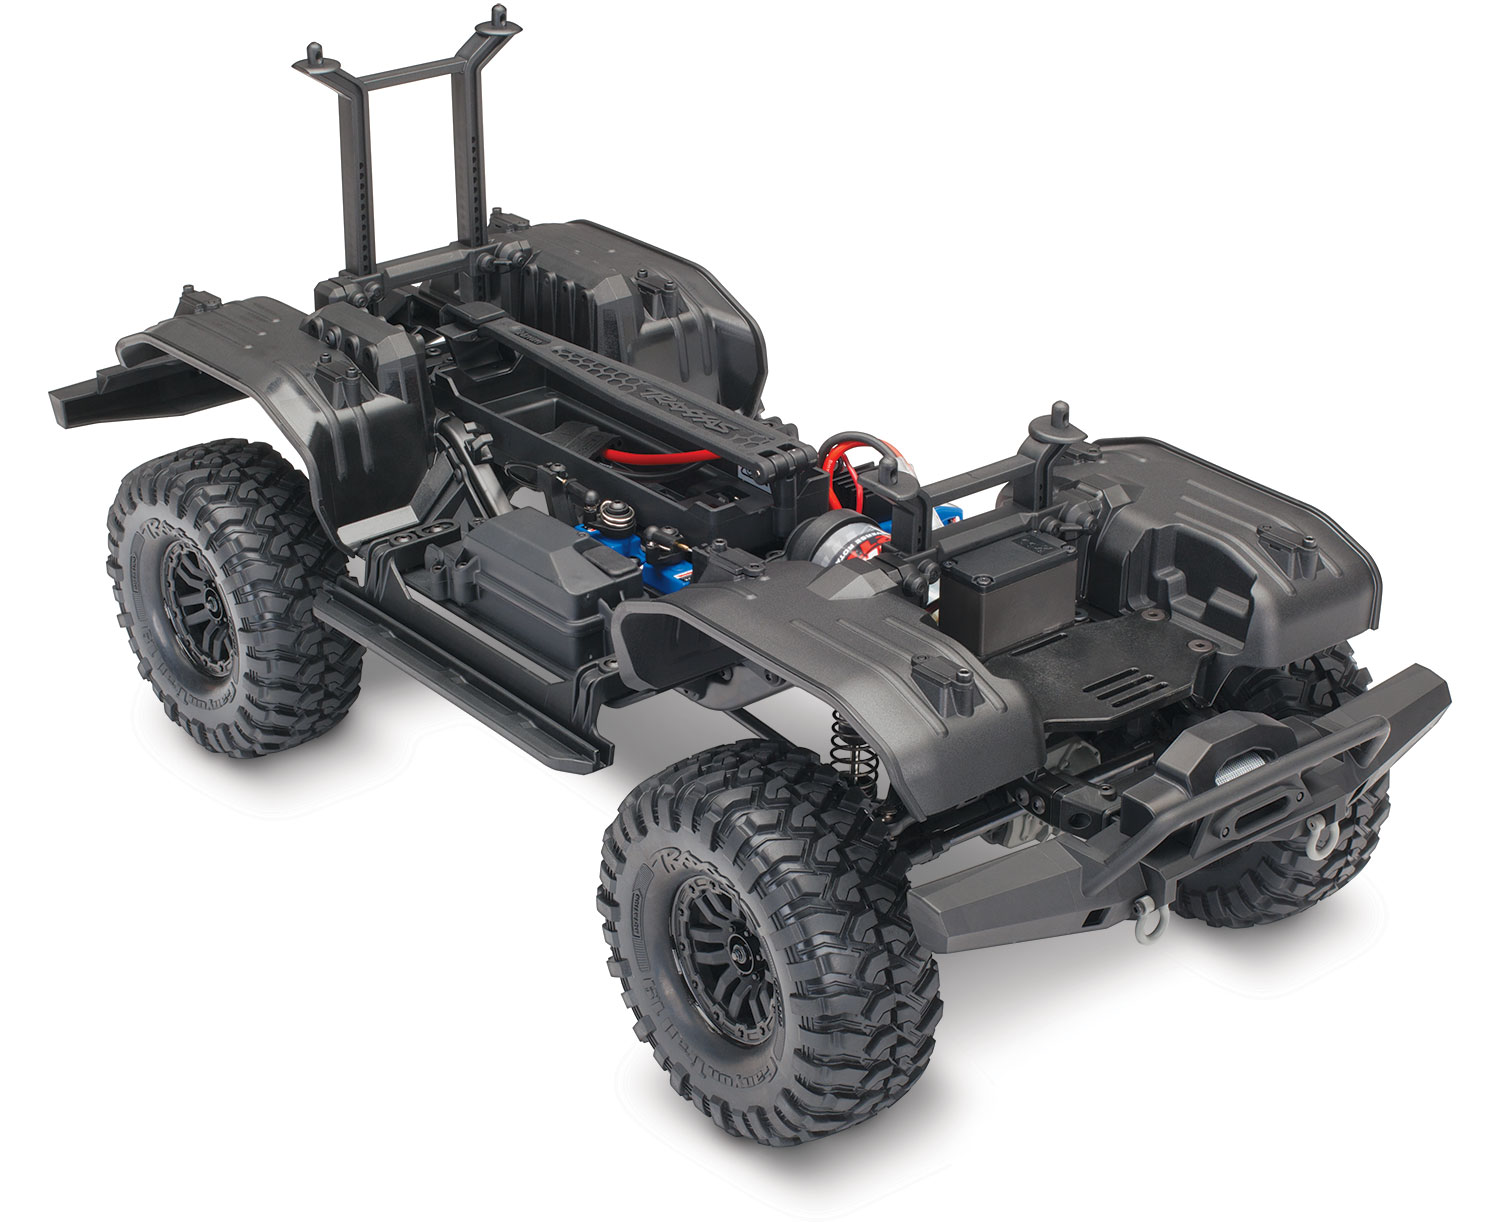
\includegraphics[width=3cm]{images/techAnalysis/TRX4.jpg}
  \caption{Traxxas TRX-4 Chassis Kit}
  \label{fig:TRX4}
\end{figure}
As can be seen on \autoref{fig:TRX4}, this kit provides a minimalistic starting point, allowing as much room as possible for our own additions and adjustments.
All support for wheels, propulsion, and steering would be taken care of with this hardware, as well as any routing of power to, and control of, all motors.
The biggest challenge would be to fit and power our own additional hardware, but, given the minimalism of the chassis, is a problem solvable by 3D-printing the needed brackets/fittings.

\subsection{AV System Platform}\label{ssec:optimalHardwareAVPlatform}
The term "AV System Platform" is, in this section, understood as a link between the engine of the car and the world the car is driving in.
This link is expected to be able to perceive (directly or indirectly) both the world around the car as well as the state of the car itself, make a decision based on all gathered information, and finally have the car perform the requested action.
To accommodate these requirements, the \textit{NVIDIA Jetson Nano Developer Kit} (depicted on \autoref{fig:JetsonNano}) would appear to be a capable platform \cite{JetsonNano}.
\begin{figure}[H]
  \centering
  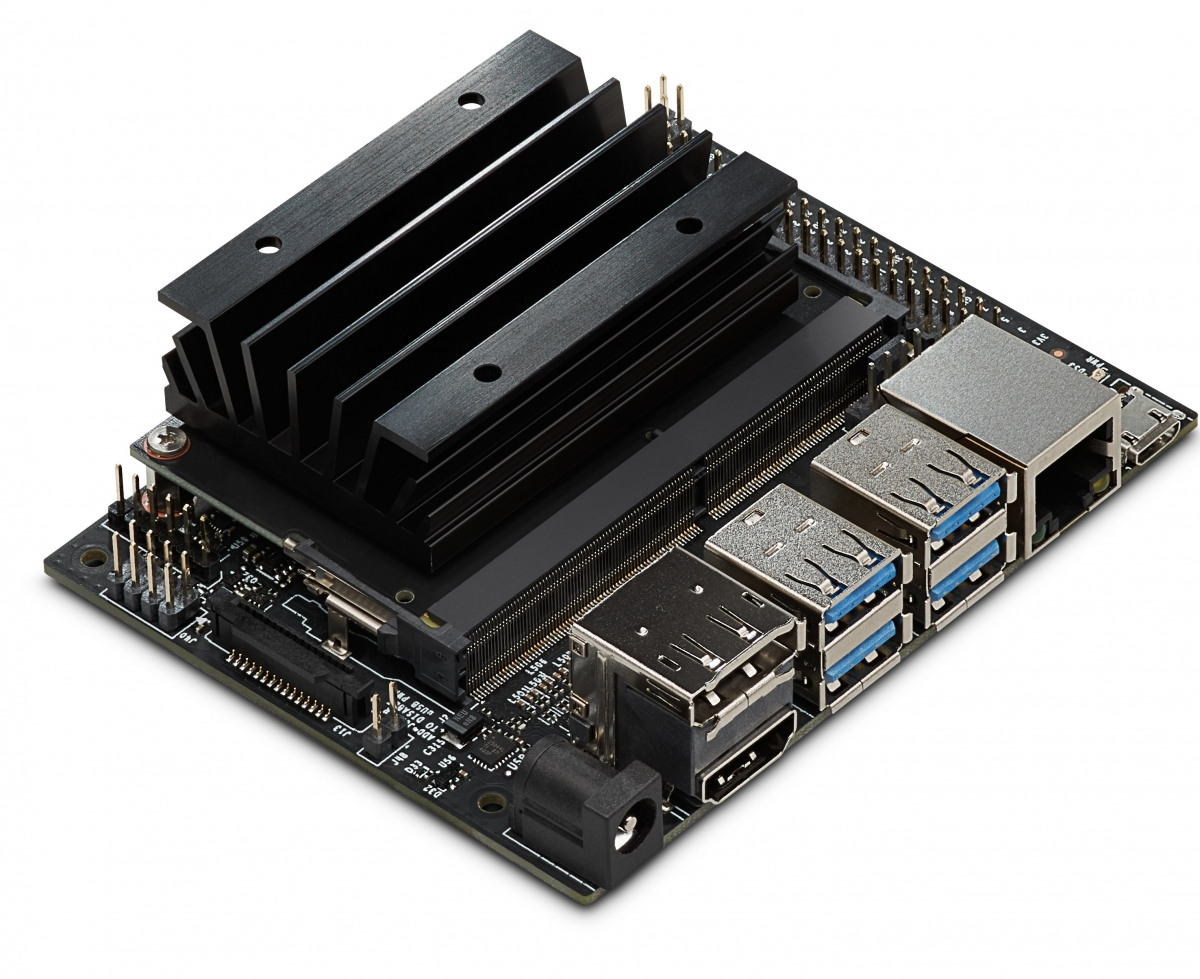
\includegraphics[width=3cm]{images/techAnalysis/JetsonNano.jpg}
  \caption{NVIDIA Jetson Nano Developer Kit}
  \label{fig:JetsonNano}
\end{figure}
As per NVIDIA's own words, the Jetson Nano is ``\textit{[...] a small, powerful computer that lets you run multiple neural networks in parallel for applications like image classification, object detection, segmentation, and speech processing.
All in an easy-to-use platform that runs in as little as 5 watts.}''
The Jetson Nano contains a dedicated 128-core Graphical Processing Unit (GPU) based on the Maxwell architecture, as well as other advantages, making it a powerful starting point.
\cite{JetsonNano}

\subsection{World Input}\label{ssec:optimalHardwareWorldInput}
As for world input to the AV system, not much is required other than ease of use and compatibility.
Since the requirements specifies the need to follow a road represented by colored lines, some sort of camera appears as an obvious candidate.
Any webcam with a USB interface should suffice, and a frequent entry when searching for the ``best USB webcam'' is the \textit{Logitech C922 Pro Stream} \cite{WebcamSearch1, WebcamSearch2, WebcamSearch3} depicted on \autoref{fig:C922}.
\begin{figure}[H]
  \centering
  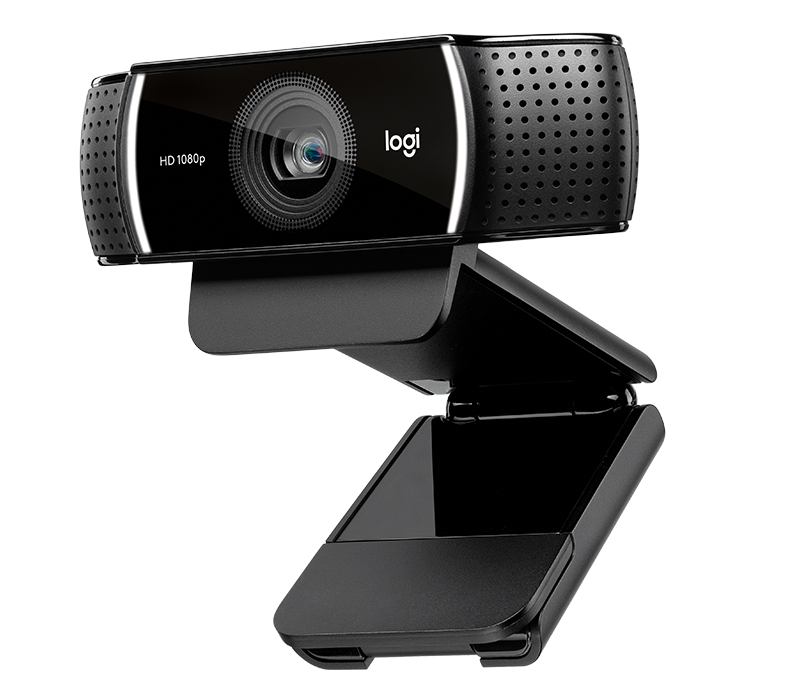
\includegraphics[width=3cm]{images/techAnalysis/c922.png}
  \caption{Logitech C922 Pro Stream}
  \label{fig:C922}
\end{figure}
This webcam is capable of capturing 60 frames per second in a resolution of 1280 times 720 pixels, which should give a satisfying amount of input data for the AV system platform to work with.
As the viewing angle for this camera is 78 degrees, more than one camera could be installed to cover a larger area.
